\section{Propagating the exceptional sets}\label{sec:descent}

We now prove Proposition~\ref{prop:density}.  Lemma~\ref{lem:residues}
provides many choices for making the numerator smaller.  Some of those
choices may land at numerators whose expansions are still unknown.  The
divisor moment in Lemma~\ref{lem:divisor} bounds how often this can happen.
An individual residue may have many possible predecessors; the moment
estimate controls their combined contribution over a small exceptional
set of residues.

\begin{proof}[Proof of Proposition~\ref{prop:density}]
Use the absolute constants and levels of Lemma~\ref{lem:residues}.  Before
choosing \(S\), fix
\[
 K_d=\frac{3D_X}{\eta},\qquad
 D_*=2D_C+D_M+1,
 \qquad r\in\N,\quad r\ge \max\{2,8K_d\},
 \qquad \alpha=1-\frac1r.
\]
All subsequent lower bounds on \(S\) may depend on these fixed constants.
In particular, the moment order \(r\) is independent of \(S\).
For sufficiently large \(S\),
\begin{equation}\label{eq:descent-depth}
 m\ge\frac{S}{2\log S},
 \qquad
 d=\left\lceil\frac{D_XS-m}{\eta m}\right\rceil
 \le \frac{2D_X}{\eta}\log S+1
 \le K_d\log S.
\end{equation}
Fix an integer \(C\) in the range of Proposition~\ref{prop:density}, and
choose the common integer \(M\) supplied by Lemma~\ref{lem:residues}.

Every fraction \(u/(MC_j)\) with \(1\le u\le X_j\) is less than one.
Indeed, if \(C_j=C\), then \(u\le X_0=e^{D_XS}<MC\); if \(C_j=1\),
then \(u\le e^S<M\).  Moreover \(C_d=1\), since \(X_d\le e^m<e^S\).
We first produce expansions at this last level, and then work backwards.

\paragraph{The last level.}
The power of two dividing \(M\) is at least \(S^{D_0}\).  For any integer
\(1\le u\le S^{D_0}\), write \(u\) in binary.  Every power \(2^k\) that
occurs divides \(M\), and
\[
 \frac{2^k}{M}=\frac1{M/2^k}.
\]
This gives an expansion of \(u/M\) with at most
\(1+D_0\log S/\log 2\) terms.

If \(S^{D_0}<u\le e^m\), the last part of Lemma~\ref{lem:residues}
gives a divisor \(t\mid M\) for which
\[
 z=\left\lceil\frac tu\right\rceil,\qquad
 h=uz-t,\qquad 0\le h\le u^{1-\eta}.
\]
The identity
\begin{equation}\label{eq:terminal-descent}
 \frac uM=\frac1{(M/t)z}+\frac1z\frac hM
\end{equation}
adds one unit fraction.  If \(h=0\), the expansion ends; otherwise an
expansion of \(h/M\) can be divided by the positive integer \(z\).
As long as the numerator remains above \(S^{D_0}\), its logarithm
decreases by a factor at most \(1-\eta\) at each step.  It starts at most
\(m\le S\), so after at most
\[
 1+\left\lceil\frac{\log S}{-\log(1-\eta)}\right\rceil
\]
steps it has either vanished or entered the binary range.  Thus an absolute constant
\(B_0\) bounds the length of every terminal expansion by \(B_0\log S\).
All denominators are integers.  Since every term is positive and the
total is less than one, every denominator is at least two.

\paragraph{Working backwards.}
Set
\[
 G_d=\{1,\ldots,\lfloor X_d\rfloor\}.
\]
At a level \(j<d\), write the list prescribed by
Lemma~\ref{lem:residues} as \((t_{j,i})_{i\in I_j}\):
it is the deterministic list when \(X_j>e^S\), and the first random
list otherwise.  Its entries may coincide; their indices are always
retained.  Having defined \(G_{j+1}\), let
\begin{equation}\label{eq:good-backwards}
 \begin{aligned}
 G_j=G_{j+1}\ \cup\ \bigl\{u\in\N:\ &1\le u\le X_j,\\
 &h_{j,t_{j,i}}(u)\in G_{j+1}\cup\{0\}
       \text{ for some }i\in I_j\bigr\}.
 \end{aligned}
\end{equation}
These sets have the asserted expansions.  For membership inherited
directly from \(G_{j+1}\), divide the known expansion by the integer
\(C_j/C_{j+1}\).  For membership obtained from a residue, put
\[
 z=\left\lceil\frac{C_jt_{j,i}}u\right\rceil,\qquad
 h=uz-C_jt_{j,i}.
\]
Then
\begin{equation}\label{eq:rescaled-descent}
 \frac{u}{MC_j}
 =\frac1{(M/t_{j,i})z}
 +\frac1{zC_j/C_{j+1}}\frac{h}{MC_{j+1}}.
\end{equation}
Both \(M/t_{j,i}\) and \(zC_j/C_{j+1}\) are positive integers.
This includes the possible transition from \(C_j=C\) to
\(C_{j+1}=1\), where the second scaling factor is \(zC\).
If \(h=0\), the second term is absent.  Otherwise it uses the known
expansion for \(h\in G_{j+1}\).  Consequently every member of \(G_j\)
has an expansion of length at most
\begin{equation}\label{eq:descent-length}
 B_0\log S+d-j.
\end{equation}

It remains to prove that almost all integers up to \(X_0\) belong to
\(G_0\).  We have built expansions whenever a residue reaches a
previously treated numerator; the following count controls all other
numerators.

\paragraph{Counting unsuccessful numerators.}
Define
\[
 H_j=\{1,\ldots,\lfloor X_j\rfloor\}\setminus G_j,
 \qquad
 \delta_j=\frac{|H_j|}{X_j}.
\]
Thus \(0\le\delta_j\le1\) and \(\delta_d=0\).
Fix \(j<d\), and abbreviate \(X=X_j\), \(Y=X_{j+1}=\rho X\).
The inclusion \(G_{j+1}\subseteq G_j\) gives
\[
 |H_j\cap[1,Y]|\le |H_{j+1}|.
\]
Apart from at most \(Xe^{-c_*m}\) exceptional integers, every
\(u\in H_j\cap(Y,X]\) has at least \(\rho|I_j|/2\) indices \(i\)
with \(h_{j,t_{j,i}}(u)\le Y\).
Each such residue lies in \(H_{j+1}\): a residue in
\(G_{j+1}\cup\{0\}\) would place \(u\) in \(G_j\).

For a fixed pair \((h,i)\), every predecessor \(u\) satisfies
\[
 u\mid C_jt_{j,i}+h,\qquad 1\le u\le X.
\]
There are at most \(d_X(C_jt_{j,i}+h)\) such predecessors.
Counting pairs with their list indices therefore yields
\begin{equation}\label{eq:bad-pair-count}
 |H_j|\le Xe^{-c_*m}+|H_{j+1}|
 +\frac{2}{\rho|I_j|}
   \sum_{i\in I_j}\ \sum_{h\in H_{j+1}}
       d_X(C_jt_{j,i}+h).
\end{equation}
Repeated values of \(t_{j,i}\) create repeated summands on both sides
of this count and require no adjustment. Figure~\ref{fig:predecessors}
shows why the index must be retained in this double count.

\begin{figure}[ht]
\centering
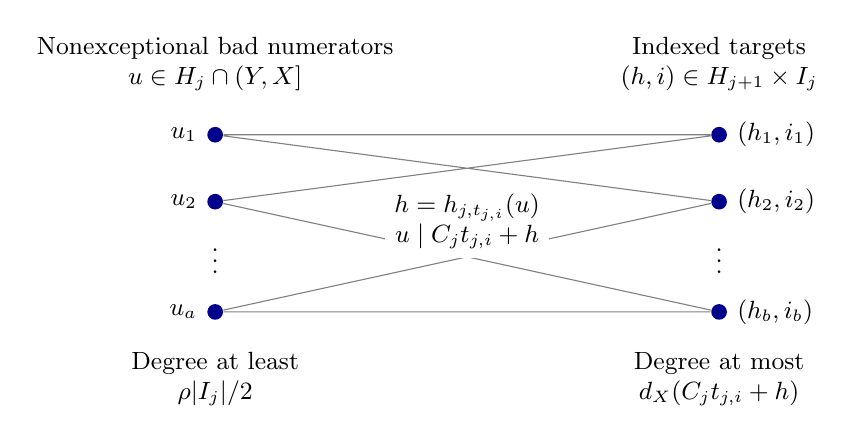
\begin{tikzpicture}[x=1cm,y=1cm,
  every node/.style={font=\small},
  point/.style={circle,fill=blue!55!black,inner sep=2pt}]
\node[align=center] at (0,1.15) {Nonexceptional bad numerators\\$u\in H_j\cap(Y,X]$};
\node[align=center] at (6.4,1.15) {Indexed targets\\$(h,i)\in H_{j+1}\times I_j$};
\node[point,label=left:$u_1$] (u1) at (0,0.25) {};
\node[point,label=left:$u_2$] (u2) at (0,-0.6) {};
\node at (0,-1.25) {$\vdots$};
\node[point,label=left:$u_a$] (ua) at (0,-2) {};
\node[point,label=right:{$(h_1,i_1)$}] (h1) at (6.4,0.25) {};
\node[point,label=right:{$(h_2,i_2)$}] (h2) at (6.4,-0.6) {};
\node at (6.4,-1.25) {$\vdots$};
\node[point,label=right:{$(h_b,i_b)$}] (hb) at (6.4,-2) {};
\draw[gray] (u1)--(h1) (u1)--(h2) (u2)--(h1) (u2)--(hb) (ua)--(h2) (ua)--(hb);
\node[fill=white,align=center] at (3.2,-0.85)
 {$h=h_{j,t_{j,i}}(u)$\\$u\mid C_jt_{j,i}+h$};
\node[align=center] at (0,-2.85) {Degree at least\\$\rho|I_j|/2$};
\node[align=center] at (6.4,-2.85) {Degree at most\\$d_X(C_jt_{j,i}+h)$};
\end{tikzpicture}
\caption{Schematic of the indexed predecessor count. Summing the right
 degrees and dividing by the left-degree lower bound gives the last term
 in \eqref{eq:bad-pair-count}. The Fourier-exception term
 $Xe^{-c_*m}$ and the inherited term $|H_{j+1}|$ are counted separately.
 Equal list values retain different indices. The drawn graph does not
 specify numerical degrees.}
\label{fig:predecessors}
\end{figure}

We check the hypotheses of Lemma~\ref{lem:divisor} before applying it.
Since \(j<d\), one has
\[
 \frac{S}{2\log S}\le m<\log X\le D_XS\le D_*S.
\]
Also
\[
 Y=Xe^{-\eta m}\ge X^{1-\eta}\ge\sqrt X,
 \qquad Y\le X.
\]
Finally, each shift \(N=C_jt_{j,i}\) is a positive integer and satisfies
\[
 N\le CM\le e^{(2D_C+D_M)S}<e^{D_*S}.
\]
Thus Lemma~\ref{lem:divisor}, with the fixed parameters \(D_*,r\),
applies uniformly at every level and to every list entry.
H\"older's inequality gives
\begin{align}
 \sum_{h\in H_{j+1}}d_X(N+h)
 &\le |H_{j+1}|^\alpha
       \left(\sum_{1\le h\le Y}d_X(N+h)^r\right)^{1/r}\notag\\
 &\le Y\,e^{S^{1/4}/r}\delta_{j+1}^{\alpha}.
 \label{eq:descent-holder}
\end{align}
This also holds when \(H_{j+1}\) is empty.
Substitution in \eqref{eq:bad-pair-count}, followed by division by \(X\),
uses \(Y=\rho X\) to cancel the factor \(1/\rho\):
\[
 \delta_j\le e^{-c_*m}+\rho\delta_{j+1}
                 +2e^{S^{1/4}/r}\delta_{j+1}^{\alpha}.
\]
Since \(\delta_{j+1}\le\delta_{j+1}^{\alpha}\), for sufficiently large
\(S\) we obtain the uniform recurrence
\begin{equation}\label{eq:density-recurrence}
 \delta_j\le\epsilon+A\delta_{j+1}^{\alpha},
 \qquad
 \epsilon=e^{-c_*m},\qquad A=e^{2S^{1/4}}.
\end{equation}

\paragraph{Iterating the recurrence.}
Our fixed choice of \(r\) ensures
\begin{equation}\label{eq:alpha-depth}
 \alpha^d
 \ge e^{-2d/r}
 \ge S^{-2K_d/r}
 \ge S^{-1/4},
\end{equation}
where we used \(-\log(1-1/r)\le2/r\) and
\eqref{eq:descent-depth}.
For nonnegative \(a,b\), the inequality
\((a+b)^\alpha\le a^\alpha+b^\alpha\) permits us to unroll
\eqref{eq:density-recurrence} from \(\delta_d=0\):
\begin{equation}\label{eq:density-unrolled}
 \delta_0\le
 \sum_{i=0}^{d-1}
 A^{(1-\alpha^i)/(1-\alpha)}\epsilon^{\alpha^i}
 \le d\exp\!\left(2rS^{1/4}-c_*mS^{-1/4}\right).
\end{equation}
Indeed, the exponent of \(A\) is at most \(r\), and
\(\alpha^i\ge\alpha^d\ge S^{-1/4}\).
The right-hand side tends to zero: the negative term has size at least
\(c_*S^{3/4}/(2\log S)\), which dominates the fixed multiple
\(2rS^{1/4}\) and \(\log d\).

For all sufficiently large \(S\), we therefore have
\[
 |H_0|\le X_0/8.
\]
Take \(G=G_0\) and \(X=X_0\).  By
\eqref{eq:descent-depth} and \eqref{eq:descent-length}, every \(u\in G\)
has an expansion of \(u/(MC)\) with at most
\((B_0+K_d)\log S\) terms.  The size bounds on \(M\) come from
Lemma~\ref{lem:residues}.  Every estimate above is uniform in the
allowed integer \(C\), and all thresholds depend only on fixed absolute
constants.  Choosing \(L=B_0+K_d\) and then one sufficiently large
absolute \(S_0\) proves Proposition~\ref{prop:density}.
\end{proof}

The proposition supplies short expansions on one common dense set of
numerators.  Section~\ref{sec:elementary} transfers this density statement
to every original fraction by writing a suitably scaled numerator as
the sum of two members of that set.
